%%%%%%%%%%%%%%%%%%%%%%%%%%%%%%%%%%%%%%%%%%%%%%%%%%%%%%%%%%%%%%%%%%%%%%
% 
% Model copied by overleaf.
%
%%%%%%%%%%%%%%%%%%%%%%%%%%%%%%%%%%%%%%%%%%%%%%%%%%%%%%%%%%%%%%%%%%%%%%

\documentclass[12pt]{article}

\usepackage{sbc-template}

\usepackage{graphicx,url}

%\usepackage[brazil]{babel}   
\usepackage[utf8]{inputenc}  

     
\sloppy

\title{ZeroMQ Distributed Message Middleware\\Uma breve abordagem}

\author{Eduardo Pedersetti José\inst{1}, Ivan Andreis\inst{1}, Leonardo S. Paula\inst{1}}

\address{Ciência da Computação -- Universidade do Vale do Rio dos Sinos (UNISINOS)\\
  Caixa Postal 15.064 -- São Leopoldo -- RS -- Brasil
\email{\{eduardoxy,ivann.andreis,leonardopaula\}@gmail.com}
}

\begin{document} 

\maketitle

\begin{abstract}
  Abstract text.
\end{abstract}
     
\begin{resumo} 
  Texto do resumo.
\end{resumo}

\section{Middleware}
A evolução das redes de computadores com o advento da internet facilitaram a ploriferação 
de aplicações distribuídas. Sabendo que as partes interessadas de uma aplicação
distribuída podem executar em diferentes locais físicos diversas vantagens podem ser
acrescidas à aplicações distribuídas, como tolerância à falhas (através de replicação) e
aumento de de performance através da paralelização de tarefas, por exemplo.

Analisando ambientes onde os Sistemas Distribuídos são executados, nota-se uma
heterogeneidade entre os dispositivos que estão se comunicando. Podem existir, em um 
mesmo Sistema Distribuído, diferentes plataformas de hardware, tecnologias de rede,
sistemas operacionais e linguagens de programação. Essas particularidades podem tornar o
desenvolvimento de um SD grande desafio  (Extraído do Livro Distributed Systems
Architecture).

É notável, portanto, que para propiciar o desenvolvimento de uma aplicação distribuida se
faz necessária uma infraestrutura adequada, que permita para o desenvolvimento e execução
de um SD. Essa infraestrutura necessária é fornecida por um middleware. Um middleware é
uma camada de software que reside entre a aplicação e a API de acesso à rede, sendo
responsável por abstrair os detalhes de rede que podem ser ignorados pela aplicação.

A rede simplesmente fornece o acesso à camada de transporte, e o acesso à ela difere
dependendo da tecnologia e da plataforma física utilizadas. O Middleware homogeniza o
acesso às redes, oferecendo serviços genéricos às aplicações. Além de interligar
diferentes domínios de tecnologias e encapsular as diferenças entre os sistemas. (Extraído
do Livro Distributed Systems Architecture)(Inserir Figura Aqui.)
Como o middleware é uma interface entre a API de acesso à rede e a aplicação, ele possui
duas visões: a visão do programador da aplicação e a visão do programador do sistema.

% Imagem da ilustração de um middleware.
\begin{figure}[ht]
\centering
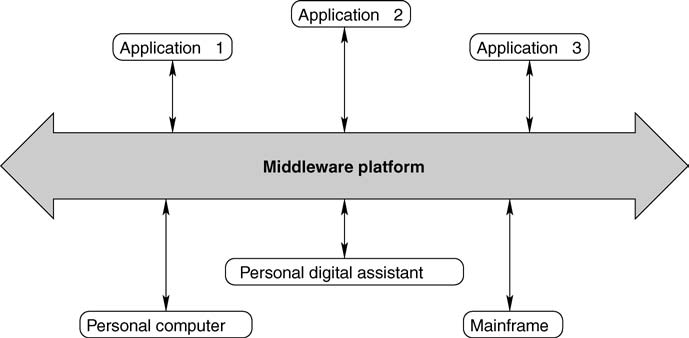
\includegraphics[width=.5\textwidth]{Img_Middleware_Arc.png}
\caption{Arquitetura básica de um middleware}
\label{fig:exampleFig1}
\end{figure}

O programador da aplicação vê o Middleware como uma ferramenta de auxílio para o
desenvolvimento de aplicações distribuídas. Estes programadores não estão interessados
como que o Middleware é implementado mas sim como obter acesso prático aos seus recursos. O Middleware é
uma caixa-preta para o programador da aplicação, com uma interface de acesso bem definida.

O programador de sistemas vai além. Para ele o Middleware é uma caixa-branca e seu
interesse maior não está em como o esta caixa interage com o mundo externo, mas sim em
como ocorrem os processos internos nela. A aplicação que utilizará o Middleware, para o
programador de sistemas, tem uma importância menor. O ponto de referência comum à ambos,
programador de sistema e de aplicações, é a interface fornecida pelo middleware que será
utilizada pelas aplicações.

\section{Um pouco sobre Filas de Mensagens}
Filas de Mensagens, ou message queues, são conhecidas tecnicamente como FIFO (First In First Out) consistem
em uma estrutura de dados bem definida e estudada. Diferentes formas de implementação de FIFO, como filas de 
prioridades e filas duplamente terminadas (deque - Double End Queue), já estão consolidadas na implementação
de algoritmos para troca de dados. A ideia de uma fila de mensagens é simples: a informação é armazenada na 
fila e é buscada quando estiver pronta ou quando o requisitante da informação à solicitar.

Embora a ideia seja simples, à implementação nem sempre é trivial. Para implementar uma fila de mensagens simples
em memória alguns problemas podem surgir, como quedas de energia elétrica ou falhas de hardware, e o conteúdo 
inteiro da fila será perdido. Quando isso ocorre o programa que está à espera de uma mensagem daquela fila 
corrompida não receberá nenhuma mensagem.

Para contornar estes problemas que se utilizam dispositivos que implementam filas de mensagens. Ao adotar um
dispositivo que gerencia uma fila de mensagem, se tem uma garantia à priori de que todas as mensagens serão 
entregues ao seu destino independentemente do que aconteça. As filas de mensagens tem um papel importantíssimo
em Sistemas Distribuídos: habilitar a comunicação assíncrona de processos.

(Colar Figura de uma Fila)

Ao invés de utilizar um componente que implemente uma fila de mensagens podem ser utilizadas abordagens como 
uma thread que gerencia uma fila de mensagens ou até diversas threads para gerenciar uma fila de mensagens.
Porém estas abordagens trazem pontos fracos. Em um sistema single-threaded a aplicação pode não ser capaz de
processar todas as requisições quando o número de clientes for muito grande. Em um sistema multi-threaded a 
aplicação pode ficar vulnerável à um ataque de negação de serviço (Distributed Denial of Service - DDoS). 
Além de que todas as informações da fila poderão ser perdidas em caso de uma falha de energia ou falha de 
hardware. Portanto é imprescindível para a execução de um sistema distribuído a utilização de um sistema de 
fila de mensagens confiável.

\section{ZeroMQ} \label{sec:firstpage}
O ZeroMQ é um software opensource apoiado por uma comunidade ativa e com suporte comercial pago. 
Ele fornece ferramentas para construção de arquiteturas centralizadas, distribuídas, pequenas ou grandes.
Pode transmitir as mensagens através de IPC, TCP, TIPC e multicast. O ZeroMQ fornece padrões como 
publish-subscriber, push-pull, e router-dealer além de mecanismos de entrada e saída de alta velocidade.

A definição formal do ZeroMQ é a seguinte: o ZeroMQ é uma biblioteca de mensagem feita para
ajudar os desenvolvedores a projetarem aplicações distribuídas e concorrentes. Embora o ZeroMQ, 
chamado daqui para frente de ZMQ, seja similar à uma fila de mensagens (ou message queue), é
importante deixar claro que ele não é um sistema de fila como o ActiveMQ, WebSphereMQ ou RabbitMQ.
O ZMQ é diferente. O ZMQ fornece todas as ferramentas necessárias para que o desenvolvedor desenvolva
o seu próprio sistema de fila de mensagens, ou seja, o ZMQ é uma biblioteca.
O ZMQ é uma biblioteca desenvolvida nativamente na linguagem C e roda em diversas plataformas. 
Atualmente ele oferece suporte à mais de vinte linguagens de programação, entre elas estão C/C++, Ruby, 
PHP, Python, Node.js entre outras.

O ZMQ é uma biblioteca simples. Operações de entrada e saída assíncronas pode enfileirar mensagens em
uma thread para tratamento de entrada e saídas. Estas threads trabalham de maneira assíncronas quando 
tratam o fluxo da rede, deixando o restante do trabalho para ser realizado pelo desenvolvedor. O ZMQ 
oferece uma interface simplificada para trabalhar com sockets se comparada às diretivas utilizadas
na linguagem C, por exemplo.

\subsection{Histórico}
Pieter Hintjens, especialista em sistemas distribuídos e responsável pela modelagem de 


\subsection{Aplicações}
\subsection{Operação}

\section{Concorrentes}

\section{Análise}
\section{Conclusão}

\section{Figures and Captions}\label{sec:figs}


Figure and table captions should be centered if less than one line
(Figure~\ref{fig:exampleFig1}), otherwise justified and indented by 0.8cm on
both margins, as shown in Figure~\ref{fig:exampleFig2}. The caption font must
be Helvetica, 10 point, boldface, with 6 points of space before and after each
caption.

\begin{figure}[ht]
\centering
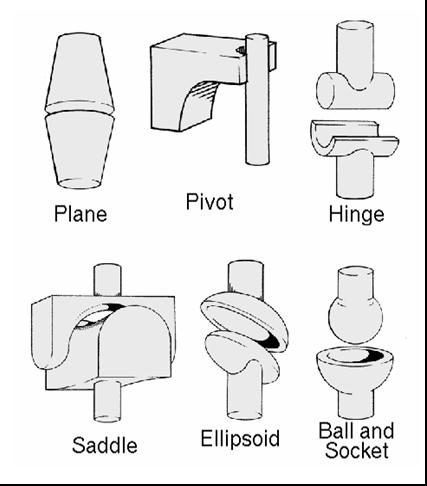
\includegraphics[width=.3\textwidth]{fig2.jpg}
\caption{This figure is an example of a figure caption taking more than one
  line and justified considering margins mentioned in Section~\ref{sec:figs}.}
\label{fig:exampleFig2}
\end{figure}

In tables, try to avoid the use of colored or shaded backgrounds, and avoid
thick, doubled, or unnecessary framing lines. When reporting empirical data,
do not use more decimal digits than warranted by their precision and
reproducibility. Table caption must be placed before the table (see Table 1)
and the font used must also be Helvetica, 10 point, boldface, with 6 points of
space before and after each caption.

\begin{table}[ht]
\centering
\caption{Variables to be considered on the evaluation of interaction
  techniques}
\label{tab:exTable1}
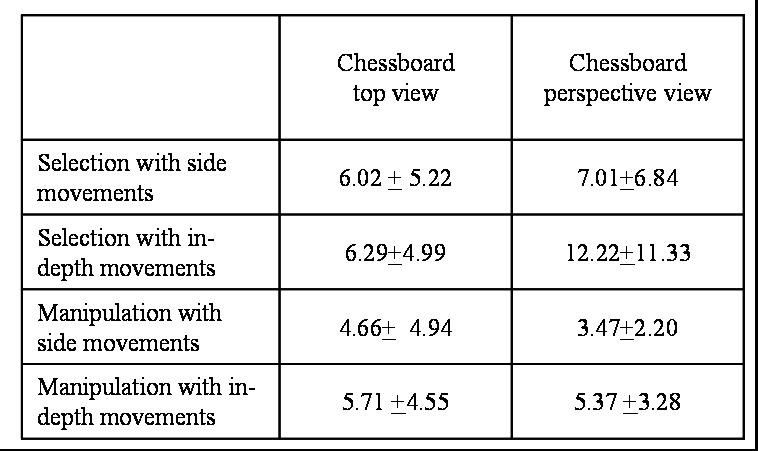
\includegraphics[width=.7\textwidth]{table.jpg}
\end{table}

\section{Images}

All images and illustrations should be in black-and-white, or gray tones,
excepting for the papers that will be electronically available (on CD-ROMs,
internet, etc.). The image resolution on paper should be about 600 dpi for
black-and-white images, and 150-300 dpi for grayscale images.  Do not include
images with excessive resolution, as they may take hours to print, without any
visible difference in the result. 

\section{References}

Bibliographic references must be unambiguous and uniform.  We recommend giving
the author names references in brackets, e.g. \cite{knuth:84},
\cite{boulic:91}, and \cite{smith:99}.

The references must be listed using 12 point font size, with 6 points of space
before each reference. The first line of each reference should not be
indented, while the subsequent should be indented by 0.5 cm.

\bibliographystyle{sbc}
\bibliography{sbc-template}

\end{document}
